\documentclass[11pt,]{article}
\usepackage[left=1in,top=1in,right=1in,bottom=1in]{geometry}
\newcommand*{\authorfont}{\fontfamily{phv}\selectfont}
  \usepackage[]{mathpazo}
  
  
  \usepackage[T1]{fontenc}
\usepackage[utf8]{inputenc}



\usepackage{abstract}
\renewcommand{\abstractname}{}    % clear the title
\renewcommand{\absnamepos}{empty} % originally center

\renewenvironment{abstract}
{{%
  \setlength{\leftmargin}{0mm}
  \setlength{\rightmargin}{\leftmargin}%
}%
  \relax}
{\endlist}

\makeatletter
\def\@maketitle{%
  \newpage
  %  \null
  %  \vskip 2em%
    %  \begin{center}%
    \let \footnote \thanks
  {\fontsize{18}{20}\selectfont\raggedright  \setlength{\parindent}{0pt} \@title \par}%
}
%\fi
\makeatother


  
  
  \setcounter{secnumdepth}{0}

      \usepackage{color}
  \usepackage{fancyvrb}
  \newcommand{\VerbBar}{|}
  \newcommand{\VERB}{\Verb[commandchars=\\\{\}]}
  \DefineVerbatimEnvironment{Highlighting}{Verbatim}{commandchars=\\\{\}}
  % Add ',fontsize=\small' for more characters per line
  \usepackage{framed}
  \definecolor{shadecolor}{RGB}{248,248,248}
  \newenvironment{Shaded}{\begin{snugshade}}{\end{snugshade}}
  \newcommand{\AlertTok}[1]{\textcolor[rgb]{0.94,0.16,0.16}{#1}}
  \newcommand{\AnnotationTok}[1]{\textcolor[rgb]{0.56,0.35,0.01}{\textbf{\textit{#1}}}}
  \newcommand{\AttributeTok}[1]{\textcolor[rgb]{0.77,0.63,0.00}{#1}}
  \newcommand{\BaseNTok}[1]{\textcolor[rgb]{0.00,0.00,0.81}{#1}}
  \newcommand{\BuiltInTok}[1]{#1}
  \newcommand{\CharTok}[1]{\textcolor[rgb]{0.31,0.60,0.02}{#1}}
  \newcommand{\CommentTok}[1]{\textcolor[rgb]{0.56,0.35,0.01}{\textit{#1}}}
  \newcommand{\CommentVarTok}[1]{\textcolor[rgb]{0.56,0.35,0.01}{\textbf{\textit{#1}}}}
  \newcommand{\ConstantTok}[1]{\textcolor[rgb]{0.00,0.00,0.00}{#1}}
  \newcommand{\ControlFlowTok}[1]{\textcolor[rgb]{0.13,0.29,0.53}{\textbf{#1}}}
  \newcommand{\DataTypeTok}[1]{\textcolor[rgb]{0.13,0.29,0.53}{#1}}
  \newcommand{\DecValTok}[1]{\textcolor[rgb]{0.00,0.00,0.81}{#1}}
  \newcommand{\DocumentationTok}[1]{\textcolor[rgb]{0.56,0.35,0.01}{\textbf{\textit{#1}}}}
  \newcommand{\ErrorTok}[1]{\textcolor[rgb]{0.64,0.00,0.00}{\textbf{#1}}}
  \newcommand{\ExtensionTok}[1]{#1}
  \newcommand{\FloatTok}[1]{\textcolor[rgb]{0.00,0.00,0.81}{#1}}
  \newcommand{\FunctionTok}[1]{\textcolor[rgb]{0.00,0.00,0.00}{#1}}
  \newcommand{\ImportTok}[1]{#1}
  \newcommand{\InformationTok}[1]{\textcolor[rgb]{0.56,0.35,0.01}{\textbf{\textit{#1}}}}
  \newcommand{\KeywordTok}[1]{\textcolor[rgb]{0.13,0.29,0.53}{\textbf{#1}}}
  \newcommand{\NormalTok}[1]{#1}
  \newcommand{\OperatorTok}[1]{\textcolor[rgb]{0.81,0.36,0.00}{\textbf{#1}}}
  \newcommand{\OtherTok}[1]{\textcolor[rgb]{0.56,0.35,0.01}{#1}}
  \newcommand{\PreprocessorTok}[1]{\textcolor[rgb]{0.56,0.35,0.01}{\textit{#1}}}
  \newcommand{\RegionMarkerTok}[1]{#1}
  \newcommand{\SpecialCharTok}[1]{\textcolor[rgb]{0.00,0.00,0.00}{#1}}
  \newcommand{\SpecialStringTok}[1]{\textcolor[rgb]{0.31,0.60,0.02}{#1}}
  \newcommand{\StringTok}[1]{\textcolor[rgb]{0.31,0.60,0.02}{#1}}
  \newcommand{\VariableTok}[1]{\textcolor[rgb]{0.00,0.00,0.00}{#1}}
  \newcommand{\VerbatimStringTok}[1]{\textcolor[rgb]{0.31,0.60,0.02}{#1}}
  \newcommand{\WarningTok}[1]{\textcolor[rgb]{0.56,0.35,0.01}{\textbf{\textit{#1}}}}
        
    \usepackage{graphicx,grffile}
\makeatletter
\def\maxwidth{\ifdim\Gin@nat@width>\linewidth\linewidth\else\Gin@nat@width\fi}
\def\maxheight{\ifdim\Gin@nat@height>\textheight\textheight\else\Gin@nat@height\fi}
\makeatother
% Scale images if necessary, so that they will not overflow the page
% margins by default, and it is still possible to overwrite the defaults
% using explicit options in \includegraphics[width, height, ...]{}
\setkeys{Gin}{width=\maxwidth,height=\maxheight,keepaspectratio}
  
    \title{Homework 3  }
  
  
  
  \author{\Large Joyce Yu Cahoon\vspace{0.05in} \newline\normalsize\emph{}  }
  
  
  \date{}

\usepackage{titlesec}

\titleformat*{\section}{\normalsize\bfseries}
\titleformat*{\subsection}{\normalsize\itshape}
\titleformat*{\subsubsection}{\normalsize\itshape}
\titleformat*{\paragraph}{\normalsize\itshape}
\titleformat*{\subparagraph}{\normalsize\itshape}


  
      
  
  \newtheorem{hypothesis}{Hypothesis}
\usepackage{setspace}

\makeatletter
\@ifpackageloaded{hyperref}{}{%
  \ifxetex
  \PassOptionsToPackage{hyphens}{url}\usepackage[setpagesize=false, % page size defined by xetex
                                                 unicode=false, % unicode breaks when used with xetex
                                                 xetex]{hyperref}
  \else
    \PassOptionsToPackage{hyphens}{url}\usepackage[unicode=true]{hyperref}
  \fi
}

\@ifpackageloaded{color}{
  \PassOptionsToPackage{usenames,dvipsnames}{color}
}{%
  \usepackage[usenames,dvipsnames]{color}
}
\makeatother
\hypersetup{breaklinks=true,
bookmarks=true,
pdfauthor={Joyce Yu Cahoon ()},
pdfkeywords = {},  
pdftitle={Homework 3},
colorlinks=true,
citecolor=blue,
urlcolor=blue,
linkcolor=magenta,
pdfborder={0 0 0}}
\urlstyle{same}  % don't use monospace font for urls

% set default figure placement to htbp
\makeatletter
\def\fps@figure{htbp}
\makeatother

\setlength{\abovedisplayskip}{.2pt}
\setlength{\belowdisplayskip}{.2pt}
\usepackage{placeins}
\usepackage{setspace}
\usepackage{chngcntr}
\usepackage{multicol}
\usepackage{lscape}
\counterwithin{figure}{section}
\counterwithin{table}{section}
\usepackage{mathrsfs}
\usepackage{mathtools}
\usepackage{multirow}
\newtheorem{theorem}{Theorem}
\usepackage[linesnumbered,algoruled,boxed,lined,commentsnumbered]{algorithm2e}
\usepackage{bm}
\usepackage{framed}
\usepackage{xcolor}
\let\oldquote=\quote
\let\endoldquote=\endquote
\colorlet{shadecolor}{orange!15}
\renewenvironment{quote}{\begin{shaded*}\quote}{\endquote\end{shaded*}}
\newcommand{\V}[1]{{\bm{{#1}}}}


% add tightlist ----------
\providecommand{\tightlist}{%
\setlength{\itemsep}{0pt}\setlength{\parskip}{0pt}}

\begin{document}

% \pagenumbering{arabic}% resets `page` counter to 1 
%
% \maketitle

{% \usefont{T1}{pnc}{m}{n}
\setlength{\parindent}{0pt}
\thispagestyle{plain}
{\fontsize{18}{20}\selectfont\raggedright 
\maketitle  % title \par  

}

{
  \vskip 13.5pt\relax \normalsize\fontsize{11}{12} 
  \textbf{\authorfont Joyce Yu Cahoon} \hskip 15pt \emph{\small }   
  
}

}






\vskip 6.5pt


\noindent  \hypertarget{section}{%
\section{6.3}\label{section}}

Let \({\bm{{Y}}}_t\) be a vector of excess returns of \(N\) assets.
Consider the multivariate linear regression model: \[
{\bm{{Y}}}_t = \alpha + \beta Y_t^m + {\bm{{\epsilon}}}_t
\] where \({\bm{{\epsilon}}}_t \sim N(0, {\bm{{\Sigma}}})\) and
\(cov(Y_t^m, \epsilon) = 0\).

\begin{enumerate}
\def\labelenumi{\arabic{enumi}.}
\tightlist
\item
  Derive the MLE for \({\bm{{\alpha}}}\) and \({\bm{{\beta}}}\). You do
  not need to derive the MLE for \({\bm{{\Sigma}}}\) since this part is
  hard. You just take for granted that \({\bm{{\hat{\Sigma}}}}\) is the
  MLE.
\item
  Show that the MLRT for the null hypothesis \(H_0\):
  \({\bm{{\alpha}}} = 0\) is: \[
  T_2 = T[\log{(|\hat{\Sigma}_0|)} - \log{(\hat{\Sigma})}]
  \] where \({\bm{{\hat{\Sigma}}}}_0\) is the MLE under \(H_0\). Give
  the expression for \({\bm{{\hat{\Sigma}}}}_0\).
\end{enumerate}

\newpage

\hypertarget{section-1}{%
\section{6.4}\label{section-1}}

Consider the multifactor model: \[
{\bm{{Y}}}_t = {\bm{{\alpha}}} + {\bm{{B}}}{\bm{{X}}}_t + {\bm{{\epsilon}}}_t
\] with observable factor \({\bm{{X}}}_t\) where
\(\mathbb{E}{\bm{{\epsilon}}}_t =0\) and
\(cov({\bm{{X}}}_t, {\bm{{\epsilon}}}_t) = 0\).

\begin{enumerate}
\def\labelenumi{\arabic{enumi}.}
\tightlist
\item
  Based on the 20 stock portfolios over a period of 60 months on the 3
  factors, it was computed that \(|{\bm{{\hat{\Sigma}}}}_0| = 2.375\)
  and \(|{\bm{{\hat{\Sigma}}}}| = 1.624\). Test if the multifactor model
  is consistent with the empirical data, \(H_0: \alpha = 0\).
\item
  Suppose that the beta's of the GE stock over the S\&P500 index
  (\(X_1\)), the size effect \(X_2\), and the book-to-market effect
  \(X_3\) are respectively 1.3, 0.3, -0.4. Assume further that over the
  last 10 years the average risk-free interest is 4\%, the average
  return of the S\&P500 is 11\%, the average difference of returns
  between the small large capitalization is 3\%, and the average
  difference of returns between the high and low book-to-market is 2\%,
  what is the expected return of the GE stock using the Fama-French
  model?
\end{enumerate}

\newpage

\hypertarget{section-2}{%
\section{6.5}\label{section-2}}

Consider the multi-factor model: \[
{\bm{{Y}}}_t = {\bm{{\alpha}}} + {\bm{{B}}}{\bm{{X}}}_t + {\bm{{\epsilon}}}_t
\] with observable factor \({\bm{{X}}}_t\).

\begin{enumerate}
\def\labelenumi{\arabic{enumi}.}
\tightlist
\item
  Suppose that the CAPM holds and over the last five years, the average
  of the risk-free interest rate is 3.5\% and the average return of the
  CRSP value-weighted index is 12.5\%. If the market \(\beta\) of a
  stock (with respect to the index) is 1.3, what is the expected return
  of the stock?
\item
  Based on 15 stock portfolios over a period of 60 months regressed on
  five factors without knowing the risk-free interest rate, it is
  computed that \(|{\bm{{\hat{\Sigma}}}}_0| = 2.425\) and
  \(|{\bm{{\hat{\Sigma}}}}| = 1.742\). Test if the multifactor model is
  consistent with the empirical data, \(H_0: \alpha = 0\).\\
\item
  Suppose that the strict multi-factor model is correct so that
  var(\({\bm{{\epsilon}}}\)) = \({\bm{{\Sigma}}}_0\) is a diagonal
  matrix and \({\bm{{X}}}_t\) and \({\bm{{\epsilon}}}_t\) are
  uncorrelated. Show how to estimate the covariance matrix of
  \({\bm{{Y}}}\) based on the past \(T\) days' data: \[
  \{({\bm{{X}}}_t, {\bm{{Y}}}_t): t = 1, \ldots, T\}
  \]
\end{enumerate}

\newpage

\hypertarget{section-3}{%
\section{6.8}\label{section-3}}

Use the Fama-French 100 portfolios in the last five years to construct 3
common factors via the PCA based on the correlation matrix. Report the
variance explained by each principle components. Now, regress each of
the Fama-French 100 portfolios on these 3 principal components and
report the distribution (histogram) of the residual variances. Report
also the distribution of the variance of these 100 portfolios over the
same time period.

\begin{Shaded}
\begin{Highlighting}[]
\NormalTok{FF100 <-}\StringTok{ }\KeywordTok{matrix}\NormalTok{(}\KeywordTok{scan}\NormalTok{(}\StringTok{"~/workspace/st790-financial-stats/hw3/100_cleaned.txt"}\NormalTok{), }
                \DataTypeTok{ncol=}\DecValTok{101}\NormalTok{, }\DataTypeTok{byrow=}\NormalTok{T)}
\NormalTok{dates <-}\StringTok{ }\NormalTok{FF100[,}\DecValTok{1}\NormalTok{] }\CommentTok{# Time period used: 1/02/12 -- 08/31/18}
\CommentTok{# get SPX information from quantmod  }
\CommentTok{# start <- as.Date("2013-01-02")}
\CommentTok{# end <- as.Date("2018-08-31")}
\CommentTok{# getSymbols("SPY", from = start, to = end) # SPY}
\CommentTok{# SPX <- SPY[,4]}
\CommentTok{# names(SPX) <- "spx"}
\CommentTok{# daily <- log(dailyReturn(SPX)+1)*100}
\CommentTok{# saveRDS(daily, "~/workspace/st790-financial-stats/hw3/spx.rds")}
\NormalTok{X <-}\StringTok{ }\KeywordTok{readRDS}\NormalTok{(}\StringTok{"~/workspace/st790-financial-stats/hw3/spx.rds"}\NormalTok{)}
\CommentTok{# match dates }
\NormalTok{D <-}\StringTok{ }\KeywordTok{time}\NormalTok{(X) }
\NormalTok{D <-}\StringTok{ }\KeywordTok{paste0}\NormalTok{(}\KeywordTok{substr}\NormalTok{(D, }\DecValTok{1}\NormalTok{, }\DecValTok{4}\NormalTok{), }\KeywordTok{substr}\NormalTok{(D, }\DecValTok{6}\NormalTok{, }\DecValTok{7}\NormalTok{), }\KeywordTok{substr}\NormalTok{(D, }\DecValTok{9}\NormalTok{, }\DecValTok{10}\NormalTok{))}
\NormalTok{D <-}\StringTok{ }\KeywordTok{as.numeric}\NormalTok{(D)}
\NormalTok{ind <-}\StringTok{ }\KeywordTok{rep}\NormalTok{(}\DecValTok{0}\NormalTok{, }\KeywordTok{length}\NormalTok{(D)) }
\ControlFlowTok{for}\NormalTok{(i }\ControlFlowTok{in} \DecValTok{1}\OperatorTok{:}\KeywordTok{length}\NormalTok{(ind))\{}
\NormalTok{  ind[i] =}\StringTok{ }\NormalTok{(}\DecValTok{1}\OperatorTok{:}\DecValTok{1427}\NormalTok{)[dates[i] }\OperatorTok{==}\StringTok{ }\NormalTok{D]}
\NormalTok{\}}
\NormalTok{dates <-}\StringTok{ }\NormalTok{dates[ind]}
\NormalTok{FF100 <-}\StringTok{ }\NormalTok{FF100[ind, ]}

\CommentTok{# PCA Analysis }
\NormalTok{Y <-}\StringTok{ }\NormalTok{FF100[,}\DecValTok{2}\OperatorTok{:}\DecValTok{101}\NormalTok{]}
\NormalTok{resid <-}\StringTok{ }\KeywordTok{resid}\NormalTok{(}\KeywordTok{lsfit}\NormalTok{(X, Y)) }\CommentTok{# take the return of SP500 out}
\CommentTok{# cor(cbind(X,resid))}
\CommentTok{# variance explained of the first three principle components}
\NormalTok{p <-}\StringTok{ }\DecValTok{100}
\KeywordTok{eigen}\NormalTok{(}\KeywordTok{cor}\NormalTok{(resid))}\OperatorTok{$}\NormalTok{values[}\DecValTok{1}\OperatorTok{:}\DecValTok{3}\NormalTok{]}
\end{Highlighting}
\end{Shaded}

\begin{verbatim}
## [1] 37.225922  8.688453  4.163726
\end{verbatim}

\begin{Shaded}
\begin{Highlighting}[]
\CommentTok{# proportion of total variability explained by the first 3 principle components}
\KeywordTok{eigen}\NormalTok{(}\KeywordTok{cor}\NormalTok{(resid))}\OperatorTok{$}\NormalTok{values[}\DecValTok{1}\OperatorTok{:}\DecValTok{3}\NormalTok{]}\OperatorTok{/}\NormalTok{p}\OperatorTok{*}\DecValTok{100}
\end{Highlighting}
\end{Shaded}

\begin{verbatim}
## [1] 37.225922  8.688453  4.163726
\end{verbatim}

\begin{Shaded}
\begin{Highlighting}[]
\CommentTok{# regress each port on these 3 principal components }
\NormalTok{a <-}\StringTok{ }\KeywordTok{eigen}\NormalTok{(}\KeywordTok{cor}\NormalTok{(resid))}\OperatorTok{$}\NormalTok{vectors[,}\DecValTok{1}\NormalTok{]}
\NormalTok{a <-}\StringTok{ }\NormalTok{a }\OperatorTok{/}\StringTok{ }\KeywordTok{sqrt}\NormalTok{(}\KeywordTok{apply}\NormalTok{(resid, }\DecValTok{2}\NormalTok{, var))     }\CommentTok{# standardize the variables}
\NormalTok{Factor1 <-}\StringTok{ }\NormalTok{resid }\OperatorTok\StringTok{ }\NormalTok{a}
\NormalTok{resid1 <-}\StringTok{ }\KeywordTok{resid}\NormalTok{(}\KeywordTok{lsfit}\NormalTok{(}\KeywordTok{cbind}\NormalTok{(X, Factor1), Y))}
\CommentTok{# get residual variances}
\NormalTok{var1 <-}\StringTok{ }\NormalTok{resid1 }\OperatorTok\StringTok{ }\KeywordTok{t}\NormalTok{(resid1)}
\KeywordTok{hist}\NormalTok{(}\KeywordTok{diag}\NormalTok{(var1), }\DataTypeTok{breaks =} \DecValTok{50}\NormalTok{)}
\end{Highlighting}
\end{Shaded}

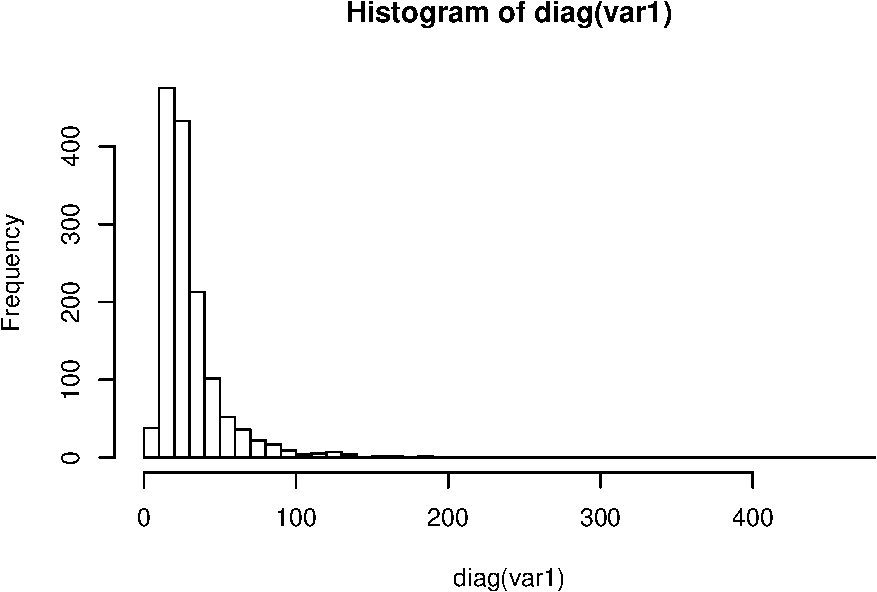
\includegraphics{hw3_files/figure-latex/unnamed-chunk-2-1.pdf}

\begin{Shaded}
\begin{Highlighting}[]
\CommentTok{# second principle component }
\NormalTok{a2 <-}\StringTok{ }\KeywordTok{eigen}\NormalTok{(}\KeywordTok{cor}\NormalTok{(resid))}\OperatorTok{$}\NormalTok{vectors[,}\DecValTok{2}\NormalTok{]}
\NormalTok{a2 <-}\StringTok{ }\NormalTok{a2 }\OperatorTok{/}\StringTok{ }\KeywordTok{sqrt}\NormalTok{(}\KeywordTok{apply}\NormalTok{(resid, }\DecValTok{2}\NormalTok{, var))   }\CommentTok{# standardize the variables}
\NormalTok{Factor2 <-}\StringTok{ }\NormalTok{resid }\OperatorTok\StringTok{ }\NormalTok{a2}
\NormalTok{resid2 <-}\StringTok{ }\KeywordTok{resid}\NormalTok{(}\KeywordTok{lsfit}\NormalTok{(}\KeywordTok{cbind}\NormalTok{(X, Factor2), Y))}
\CommentTok{# get residual variances}
\NormalTok{var2 <-}\StringTok{ }\NormalTok{resid2 }\OperatorTok\StringTok{ }\KeywordTok{t}\NormalTok{(resid2)}
\KeywordTok{hist}\NormalTok{(}\KeywordTok{diag}\NormalTok{(var2), }\DataTypeTok{breaks =} \DecValTok{50}\NormalTok{)}
\end{Highlighting}
\end{Shaded}

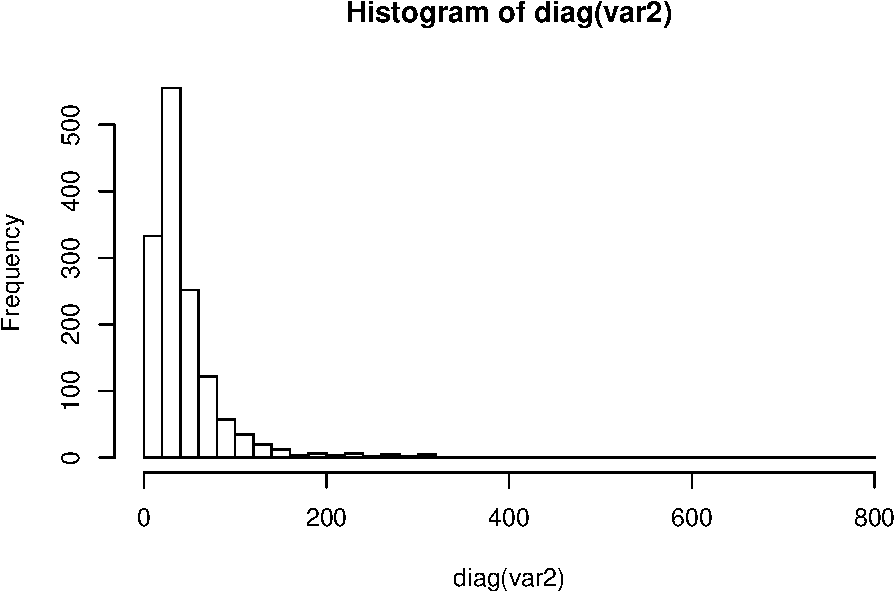
\includegraphics{hw3_files/figure-latex/unnamed-chunk-2-2.pdf}

\begin{Shaded}
\begin{Highlighting}[]
\CommentTok{# third principal components }
\NormalTok{a3 <-}\StringTok{ }\KeywordTok{eigen}\NormalTok{(}\KeywordTok{cor}\NormalTok{(resid))}\OperatorTok{$}\NormalTok{vectors[,}\DecValTok{3}\NormalTok{]}
\NormalTok{a3 <-}\StringTok{ }\NormalTok{a3 }\OperatorTok{/}\StringTok{ }\KeywordTok{sqrt}\NormalTok{(}\KeywordTok{apply}\NormalTok{(resid, }\DecValTok{2}\NormalTok{, var))   }\CommentTok{# standardize the variables}
\NormalTok{Factor3 <-}\StringTok{ }\NormalTok{resid }\OperatorTok\StringTok{ }\NormalTok{a3}
\NormalTok{resid3 <-}\StringTok{ }\KeywordTok{resid}\NormalTok{(}\KeywordTok{lsfit}\NormalTok{(}\KeywordTok{cbind}\NormalTok{(X, Factor3), Y))}
\CommentTok{# get residual variances}
\NormalTok{var3 <-}\StringTok{ }\NormalTok{resid3 }\OperatorTok\StringTok{ }\KeywordTok{t}\NormalTok{(resid3)}
\KeywordTok{hist}\NormalTok{(}\KeywordTok{diag}\NormalTok{(var3), }\DataTypeTok{breaks =} \DecValTok{50}\NormalTok{)}
\end{Highlighting}
\end{Shaded}

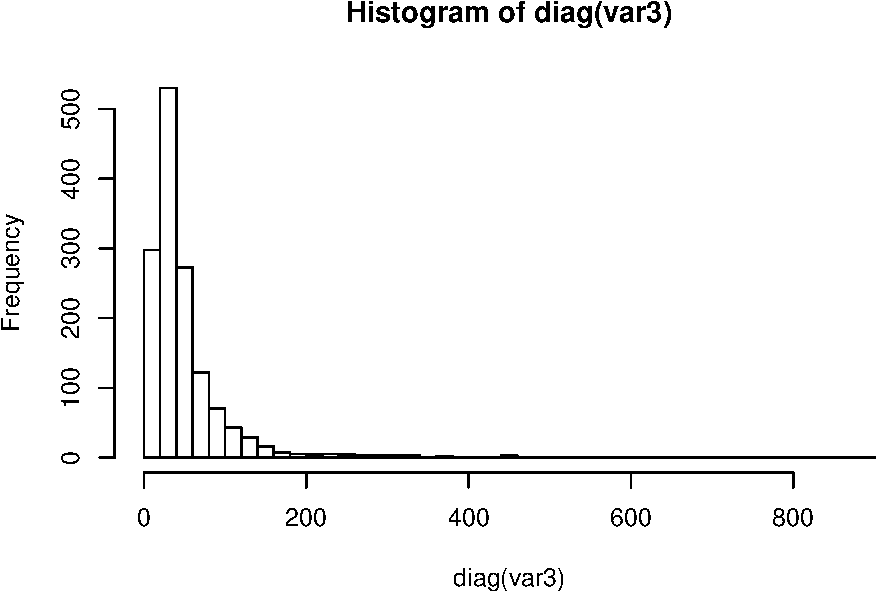
\includegraphics{hw3_files/figure-latex/unnamed-chunk-2-3.pdf}

\begin{Shaded}
\begin{Highlighting}[]
\CommentTok{# dist of variance of these 100 portfolios }
\KeywordTok{hist}\NormalTok{(}\KeywordTok{apply}\NormalTok{(Y, }\DecValTok{2}\NormalTok{, var), }\DataTypeTok{breaks =} \DecValTok{50}\NormalTok{) }
\end{Highlighting}
\end{Shaded}

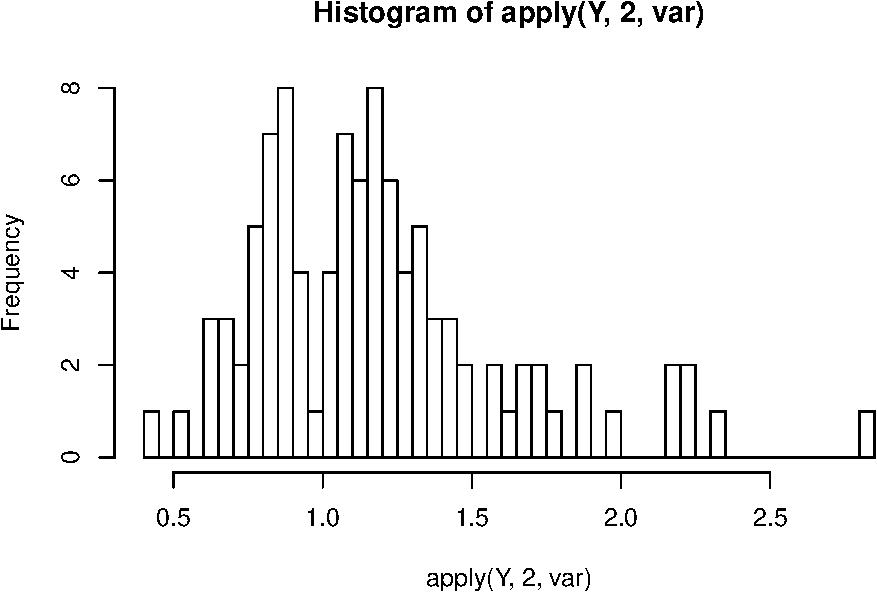
\includegraphics{hw3_files/figure-latex/unnamed-chunk-2-4.pdf}

\begin{Shaded}
\begin{Highlighting}[]
\CommentTok{# use Rsq }
\CommentTok{# Rsq1 <- 1-apply(resid1, 2, var)/apply(Y,2,var)}
\CommentTok{# hi st(Rsq1)}
\end{Highlighting}
\end{Shaded}
\newpage
\singlespacing 
\end{document}
